% -----------------------------------------------
% Template for ISMIR Papers
% 2018 version, based on previous ISMIR templates

% Requirements :
% * 6+n page length maximum
% * 4MB maximum file size
% * Copyright note must appear in the bottom left corner of first page
% * Clearer statement about citing own work in anonymized submission
% (see conference website for additional details)
% -----------------------------------------------

\documentclass{article}
\usepackage{ismir,amsmath,cite,url}
\usepackage{graphicx}
\usepackage{color}
\usepackage{microtype}
\usepackage{units}
\usepackage{graphicx}
\usepackage{multirow}
\usepackage{paralist}
%\usepackage[keeplastbox]{flushend}
\usepackage{paralist}
\usepackage{tabularx}

% Title.
% ------
\title{From labeled to unlabeled data -- on the data challenge in automatic drum transcription}

% Note: Please do NOT use \thanks or a \footnote in any of the author markup

% Single address
% To use with only one author or several with the same address
% ---------------
%\oneauthor
% {Chih-Wei Wu and Alexander Lerch}
% {Center for Music Technology, Georgia Institute of Technology\\ {\tt \{ cwu307, alexander.lerch\}@gatech.edu}}

% Two addresses
% --------------
%\twoauthors
%  {First author} {School \\ Department}
%  {Second author} {Company \\ Address}

%% To make customize author list in Creative Common license, uncomment and customize the next line
%  \def\authorname{First Author, Second Author}


% Three addresses
% --------------
\threeauthors
  {First Author} {Affiliation1 \\ {\tt author1@ismir.edu}}
  {Second Author} {\bf Retain these fake authors in\\\bf submission to preserve the formatting}
  {Third Author} {Affiliation3 \\ {\tt author3@ismir.edu}}

%% To make customize author list in Creative Common license, uncomment and customize the next line
%  \def\authorname{First Author, Second Author, Third Author}

% Four or more addresses
% OR alternative format for large number of co-authors
% ------------
%\multauthor
%{First author$^1$ \hspace{1cm} Second author$^1$ \hspace{1cm} Third author$^2$} { \bfseries{Fourth author$^3$ \hspace{1cm} Fifth author$^2$ \hspace{1cm} Sixth author$^1$}\\
%  $^1$ Department of Computer Science, University , Country\\
%$^2$ International Laboratories, City, Country\\
%$^3$  Company, Address\\
%{\tt\small CorrespondenceAuthor@ismir.edu, PossibleOtherAuthor@ismir.edu}
%}
%\def\authorname{First author, Second author, Third author, Fourth author, Fifth author, Sixth author}

\newcommand{\comment}[1]{{\textcolor{blue}{#1}}}

\sloppy % please retain sloppy command for improved formatting

\begin{document}

%
\maketitle
%
\begin{abstract}
Automatic Drum Transcription (ADT), like many other music information retrieval tasks, has made progress in the past years through the integration of machine learning and audio signal processing techniques. However, with the increasing popularity of data-hungry approaches such as deep learning, the insufficient amount of data becomes more and more a challenge that concerns the generality of the resulting models and the validity of the evaluation. To address this challenge in ADT, this paper first examines the existing labeled datasets and how representative they are of the research problem. Next, the possibilities of using unlabeled data to improve general ADT systems are explored. Specifically, two paradigms that harness information from unlabeled data, namely feature learning and student-teacher learning, are applied to two major types of ADT systems. All systems are evaluated on four different drum datasets. The results highlight the necessity of more and larger annotated datasets and indicate the feasibility of exploiting unlabeled data for improving ADT systems.
\end{abstract}

%
\section{Introduction}\label{sec:introduction}
%% how much data is enough?
%``How much data is enough?" is a commonly asked question in machine learning practices. Despite being straightforward at the first glance, this question entails a complicated problem referred to as \textit{Sample Size Determination} in the early theoretical study \cite{Raudys1991}, and it is difficult to answer without heuristics and task-dependent insights. As a result, the availability of data is constantly listed as one of the top challenges in the Music Information Retrieval (MIR) literature (e.g., Automatic Music Transcription (AMT) \cite{Benetos2013} and general MIR research \cite{Schedl2014}).

% labeled data in ADT was not enough
% MIREX 2017, performance of the systems varies quite a lot across different datasets, indicating the potential problem of generality
% attempts to do data-augmentation
% we need more data 
Automatic drum transcription (ADT), a sub-task of Automatic Music Transcription (AMT) \cite{Benetos2013} that concerns the extraction of drum events from music signals, witnesses a growth in data-driven approaches such as deep learning in recent years \cite{Vogl2016, Southall2016, Vogl2017_icassp, Southall2017, Vogl2017_ismir}. The majority of these ADT studies that focus on polyphonic mixtures use the popular ENST-Drums dataset \cite{Gillet2006_enst} for development by splitting the dataset into different subsets for training, validation, and testing purposes. Nevertheless, the limited amount of labeled data and its potential impact in the context of ADT are rarely discussed. 
The heavy reliance on one dataset leads to two major concerns: 
\begin{inparaenum}[(i)]
	\item   the model could easily overfit the data, which questions its generality, and
    \item   the evaluation results could be overly optimistic due to the small sample size of the split. 
\end{inparaenum} 
To avoid these pitfalls, larger datasets and cross-dataset evaluation are necessary. This need has been identified by researchers and has been addressed with newly released annotated datasets such as MDB-Drums \cite{Southall2017_mdb} and RBMA \cite{Vogl2017_ismir}. These new data enable us to revisit ENST-Drums and re-examine the representativeness of this widely-used dataset through a unified comparison. 

% the challenge leads to the question: 
% to answer this question 
Motivated by the above mentioned issues concerning the data in ADT, this paper aims to address the challenge from two different angles,
\begin{inparaenum}[(i)]
	\item examining the effectiveness of the existing datasets and
	\item investigating additional resources (e.g., unlabeled data) and techniques for supporting the development of general ADT systems.
\end{inparaenum} 
% the contribution and structure of the paper
The contributions of this work include: first, the examination of four different datasets, highlighting the importance of data diversity. Second, the evaluation of two paradigms for integrating unlabeled data to two major types of ADT systems. Third, the demonstration of potential improvements of both types of ADT systems on different drum instruments using unlabeled data.

%\comment{Don't you think these are a bit vague? Especially the last}
% agree... but i dont' know how to address this either....

%The rest of the paper is structured as follows: in Sect.~\ref{sec:relatedwork}, the related work is presented. Sect.~\ref{sec:method} introduces the technical details of the proposed methods, followed by the description of the datasets, experiment setup, and the evaluation results in Sect.~\ref{sec:experiment}. Finally, the conclusion and future directions are given in Sect.~\ref{sec:conc}.\\ 

%
\section{Related Work}
\label{sec:relatedwork}
%
\subsection{Automatic Drum Transcription}
% talk about automatic drum transcription
% define ADT a little bit
% the focus on HH BD SD
% polyphonic mixtures

The task of automatic drum transcription can be described as converting drum related audio events into music notation. 
%Similar to melody extraction \cite{Salamon2014}, which finds the dominant pitch values and provides information about the melodic content, ADT extracts the drum sequences and contributes to the understanding of rhythmic aspect of music. 
Most of the early ADT systems, as summarized by FitzGerald and Paulus \cite{FitzGerald2006}, detect onsets of HiHat (HH), Bass Drum (BD), and Snare Drum (SD) in drum only recordings. 
Recently, this focus has shifted towards transcribing drums in polyphonic mixtures comprised of both drum and melodic instruments. Following these conventions, this paper defines the ADT task as detecting HH, BD, and SD in polyphonic mixtures. 

Generally speaking, the existing ADT systems can be categorized into four types according to the literature \cite{Gillet2008_taslp, Paulus09_DrumStructure_PhD}. These are
\begin{inparaenum}[(i)]
	\item \textit{Segment and Classify}: following the standard pattern recognition pipeline, these approaches extract audio features from detected onset locations and classifies them with pre-trained models; this is a popular approach with many proposed systems using different combinations of classifiers and features \cite{SteelantTDBLM05_DrumTransSVM_Chapter, Gillet2008_taslp, SouzaBN15_CymbalClassi_IJCNN, Gajhede2016},
	\item \textit{Separate and Detect}: deriving activation functions from recordings to represent the activities of each drum, these systems subsequentially perform onset detection on these activation functions to locate drum hits; approaches include matrix factorization methods such as Non-negative Matrix Factorization (NMF) \cite{DittmarG14_DrumTranscription_DAFX, Roebel2015, Wu2015_ismir} and deep-learning-based methods such as Recurrent Neural Networks (RNNs) \cite{Southall2016, Vogl2016, Vogl2017_icassp} and Convolutional Neural Networks (CNNs) \cite{Southall2017, Vogl2017_ismir},
	\item \textit{Match and Adapt}: identifying drum events by comparing with a set of pre-defined templates, these systems often iteratively update the templates \cite{YoshiiGO07_DrumTrans_IEEE-TASLP}, and
	\item \textit{HMM-based Recognition}: modeling the temporal connections between drum events using probabilistic models such as Hidden Markov Models (HMMs), these models try to identify the underlying drum sequence by using the Viterbi algorithm \cite{PaulusK09_DrumTransHMM_JASMP, Dzhambazov14_DrumTransHMM_AES}. 
\end{inparaenum} 

To date, the majority of the existing ADT systems fall into the categories of \textit{Segment and Classify} and \textit{Separate and Detect}. Both these types of systems, despite having the fundamental differences, use data-driven methods and could potentially face the challenge described in Sect.~\ref{sec:introduction}.
Therefore, in this paper, we considered both types of systems in our experiments.

\subsection{Learning from Unlabeled Data}
\label{subsec:learnFromUnlabeledData}
% talk about learning from unlabeled data
To address the data challenge in MIR tasks, techniques that build upon the existing labeled data have been proposed. For example, in \textit{transfer learning} \cite{Choi2017a}, a deep neural network trained on a task that has sufficient data can be used to derive features for another task with limited data. This method alleviates the data insufficiency by re-using the effective models in the similar domains. \textit{Data augmentation}, a technique to increase diversity of training data through music-related deformations (e.g., time-stretching, pitch shifting, or distortion) and synthesis, has been successfully applied in MIR tasks \cite{Mcfee2015} and in ADT specifically \cite{Wu2016, Vogl2017_icassp}. However, these techniques still require a reasonably sized correctly annotated dataset as a starting point, which can be a challenge in certain scenarios. 
\begin{figure}
\centering
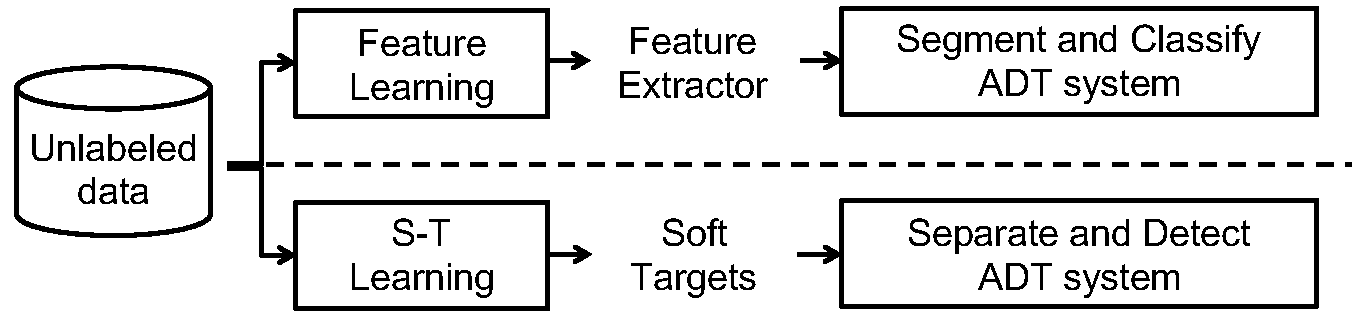
\includegraphics[width = \columnwidth]{./figs/paradigms_overview.pdf}
\caption{The overview of the evaluated paradigms for integrating unlabeled data to two major ADT approaches}
\label{fig:overview}
\end{figure}

Another direction for addressing the data scarcity is to use unlabeled data. Intuitively, a large collection of unlabeled data can be helpful in deriving more generalized features. This is the main concept of unsupervised \textit{feature learning}, and it can be implemented with algorithms such as Sparse Coding \cite{Raina2007a}, Deep Belief Networks \cite{Hamel2010}, and Auto-encoders \cite{Masci2011}. More recently, the \textit{student-teacher learning} paradigm has also emerged as an interesting concept to incorporate unlabeled data. Referred by Hinton et al.~as ``knowledge distillation'' \cite{Hinton2015}, this paradigm transfers the knowledge of a teacher model to a student model using the soft-targets generated by the teacher. As opposed to learning from the hard targets (i.e., ground truth), the student learns from the ``dark knowledge'' residing in the soft-targets, which can be created using either labeled or unlabeled data \cite{Li2014}. A successful student model can reduce the complexity of the original teacher model without significant performance loss. Some studies even report superior performance of the student models \cite{Cui2017,Watanabe2017, Wu2017}. Overall, methods that work directly with unlabeled data obviously have less dependency on existing labeled data and have shown promise for future applications. 


%
\section{Method}
\label{sec:method}
% first, start with an overview figure that shows the main idea of this paper on integrating unlabeled data
\subsection{Overview}

To connect general ADT systems to the abundant resources of unlabeled data, this paper investigates the application of \textit{feature learning} and \textit{student-teacher learning} to \textit{Segment and Classify}-based and \textit{Separate and Detect}-based ADT systems, respectively. \figref{fig:overview} shows the two paradigms for integrating unlabeled data to ADT systems as investigated in this paper. The feature learning paradigm is designed for \textit{Segment and Classify}-based ADT systems. In this paradigm, the unlabeled data is used to derive a feature extractor using an unsupervised feature learning algorithm. The resulting feature extractor is then integrated into a generic \textit{Segment and Classify} ADT framework. The student-teacher learning paradigm is suitable for \textit{Separate and Detect}-based ADT systems. This paradigm uses teacher models and unlabeled data to generate soft-targets; these soft-targets play the important role of connecting any \textit{Separate and Detect}-based system with unlabeled data and enable the training of the student model. In the following sections, more details of both paradigms are presented. 

\subsection{Feature Learning}
\label{subsec:featureLearning}
% zoom in to feature learning based method


\begin{figure}
\centering
\includegraphics[width = \columnwidth]{./figs/featurelearningSys.pdf}
\caption{The flowchart of the feature learning paradigm for ADT}
\label{fig:featureLearningFlow}
\end{figure}

\begin{figure}
\centering
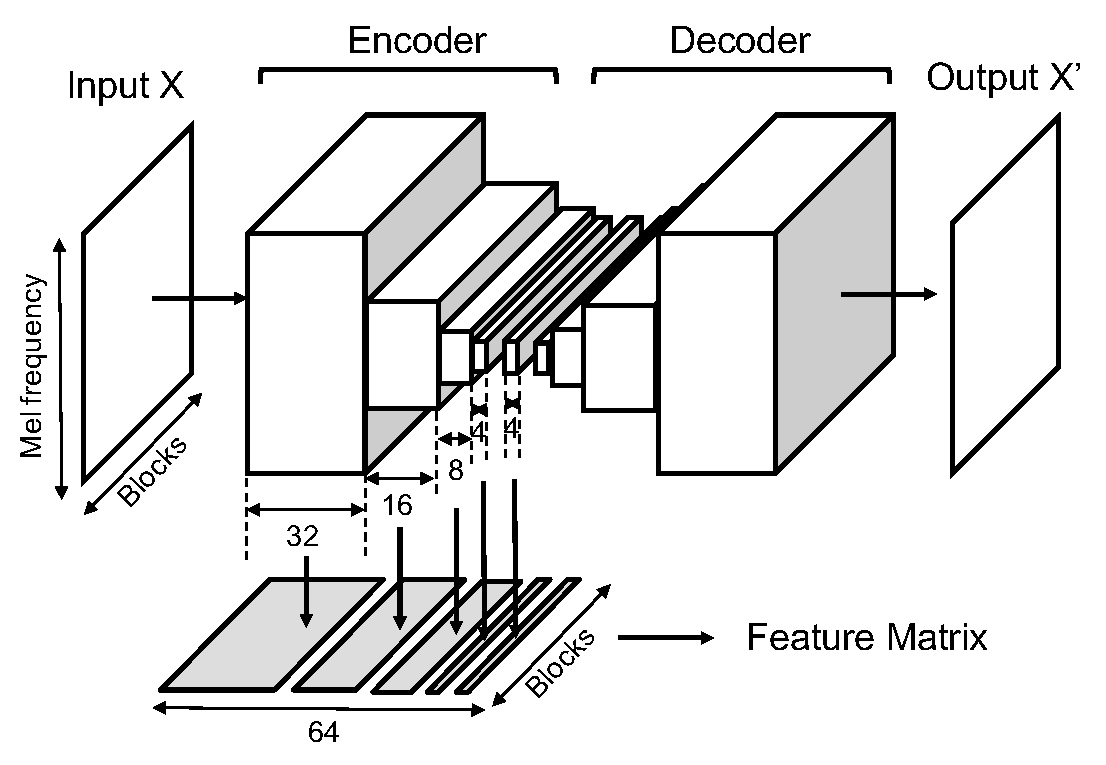
\includegraphics[width = \columnwidth]{./figs/caeStructure.pdf}
\caption{The architecture of the proposed CAE for unsupervised feature learning. The input $X$ is a $128 \times N$ Mel-spectrogram.}
\label{fig:caeStructure}
\end{figure}

The flowchart in Fig.~\ref{fig:featureLearningFlow} shows the feature learning paradigm for ADT, including both training and testing. The training phase starts with the training of a feature extractor using the unlabeled data. Specifically, we use a Convolutional Auto-encoder (CAE) as the feature extractor. A generic \textit{Segment and Classify}-based ADT system is then constructed with the following steps: first, the features are extracted from the audio signals using the pre-trained feature extractor. Second, the onset locations are determined by using the ground truth annotations while training. Finally, the feature vectors around the onset locations are collected and used to train three binary classifiers for HH, BD, and SD, respectively. The classifiers used in this paper are Support Vector Machines (SVMs). In the testing phase, the same pipeline is followed except for the onset detection step, which uses an onset detector instead of the ground truth locations. Finally, the presence of each drum can be predicted using the pre-trained SVMs. 

The architecture of the CAE in this paper is shown in Fig.~\ref{fig:caeStructure}. The input $X$ of the CAE is a Mel-spectrogram, and the output $X'$ is the reconstruction of $X$. The encoder consists of four convolutional layers with \{32, 16, 8, 4\} channels of $3 \times 3$ kernels, accordingly. Each convolutional layer is followed by a batch normalization layer and a max-pooling layer of (2, 1). This design maintains the temporal resolution, allowing the extraction of block-wise features. 
The bottleneck layer is also a convolutional layer with 4 channels of $3 \times 3$ kernels. All non-linear units are Rectified Linear Units (ReLUs).
The structure of the decoder is symmetric to the encoder with the max-pooling layers replaced by the up-sampling layers.  
The CAE is trained to minimize the Mean Squared Error (MSE) between $X$ and $X'$ using a gradient-descent-based optimization process, and the number of training epochs is $30$. 

% this architecture keeps the temporal resolution intact, allowing the extraction of frame-wise features
% talk about how we get the features and feature splicing 
The feature extraction process, as shown in Fig.~\ref{fig:caeStructure}, is inspired by the method proposed by Choi et al.~\cite{Choi2017a}: first, the intermediate outputs from all the layers in the encoder (including the bottleneck layer) are computed. Next, these outputs are aggregated across the Mel-frequency axis through averaging. Finally, the aggregated outputs are stacked into a $64 \times N$ feature matrix, where $N$ is the number of blocks. %\comment{you mean neighboring?}
To derive the final feature vector at each block, the feature vectors from the current block and the following two blocks are spliced together to capture the temporal variations of the event. This leads to a final feature vector with a dimensionality $d = 3 \times F$, in which $F$ is the number of features (i.e., 64). 
% for each layer, average pooling is applied to summarized the activation map across different channels. The resulting vectors from all layers in the encoder part are stacked and used as the final feature matrix. Splicing 

In addition to the learned features, a set of baseline features consisting of 20 Mel Frequency Cepstral Coefficients (MFCCs) and their first and second derivatives is also included in this paradigm. As a result, the baseline feature vector has a dimensionality $d = 3 \times 60 = 180$ after the feature splicing. 

\subsection{Student-Teacher Learning}
\label{subsec:studentTeacher}
% zoom in to student teacher learning method

\begin{figure}
\centering
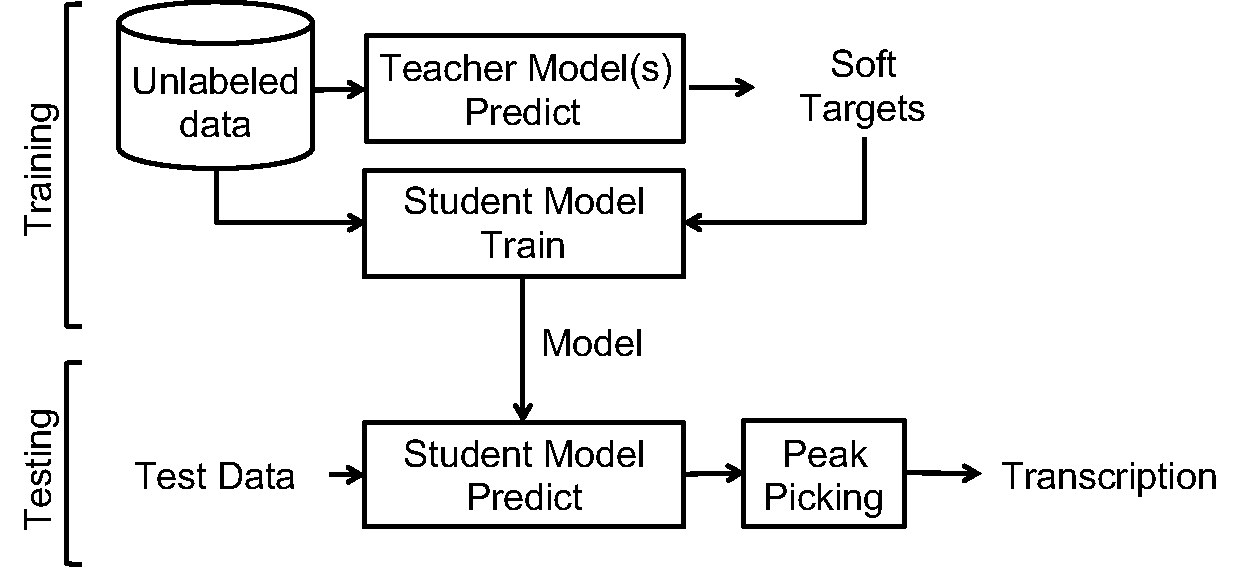
\includegraphics[width = \columnwidth]{./figs/studentTeacherSys.pdf}
\caption{The flowchart of the student-teacher learning paradigm for ADT}
\label{fig:studentTeacherFlow}
\end{figure}

Figure~\ref{fig:studentTeacherFlow} shows the flowchart of the student-teacher learning paradigm for ADT. In the training phase, the teacher models are used to analyze the unlabeled data and generate the soft-targets. These soft-targets, used as pseudo ground truth to train a student model, contain the activation functions for the different drums. 
When multiple teachers are presented, the student model can be trained by iteratively passing the unlabeled data and its corresponding soft-targets from each teacher. The student model is trained by minimizing the MSE between the soft-targets and the model outputs. 
In the testing phase, the trained student model processes the test data and generates the corresponding activation functions. The estimated locations of drum hits are identified with a simple peak picking process. 

The configuration and parametrization of this evaluated paradigm generally follows the setup described in \cite{Wu2017}. This includes two teacher models based on Partially-fixed NMF (PFNMF) \cite{Wu2015_ismir} and one student model using a fully-connected, feed-forward Deep Neural Network (DNN). The soft-targets are scaled to a numerical range between 0 and 1 using min-max scaling across the training data for each instrument in order to ensure their compatibility with the outputs from the student DNN. 
% training
% testing 
% teacher and student models
% output are normalized to {0, 1}
\subsection{Implementation}
% for feature learning part
% librosa
% madmom
% scikit-learn
% for student teacher part
% Nmftoolbox
% stft librosa
% all neural networks are 
The main input representations for both paradigms are derived from the magnitude spectrogram of the Short Time Fourier Transform (STFT), which is computed using a block size of 2048 and a hop size of 512 samples with Hann window. All of the audio signals are normalized to a range between 1 and -1, down-mixed to mono, and resampled to \unit[44.1]{kHz} prior to the computation of STFT. %\comment{normalization?}

For the feature learning paradigm, both the Mel-spectrogram in dB scale with 128 bins and the MFCCs are computed using librosa\footnote{https://librosa.github.io, last access 2018/03/27}, a Python library for audio signal processing. The onset detection is implemented using the \textit{CNNOnsetProcessor} from Madmom\footnote{https://madmom.readthedocs.io/en/latest/, last access 2018/03/27}. Additionally, the implementation of Linear SVMs from scikit-learn\footnote{http://scikit-learn.org/stable/, last access 2018/03/27}, a Python library for machine learning, is used. A grid search on the penalty parameter $C$ within \{0.1, 1, 10, 100, 1000\} is performed to optimize the performance of the SVMs. 

For student-teacher learning paradigm, the teacher models are implemented using the PFNMF function from NmfDrumToolbox\footnote{https://github.com/cwu307/NmfDrumToolbox, last access 2018/03/27}. The peak-picking parameters are set to the same as in the original paper \cite{Wu2017}.

The neural networks in both paradigms are implemented using Keras\footnote{https://keras.io, last access 2018/03/27} and the Tensorflow \cite{Abadi2016} backend. The weights are randomly initialized with normal distributions, and the parameters of the optimizers are set to default. The source code used in this paper is available on Github \footnote{http://dummy.link}.

\section{Experiment}
\label{sec:experiment}

\subsection{Unlabeled Data}

The unlabeled dataset in this paper is built using the source code provided in \cite{Wu2017}; this tool allows the compilation of a list of songs from the Billboard Chart\footnote{https://www.billboard.com/charts, last access 2018/03/27} and the retrieval of these songs from Youtube. This dataset consists of six musical genres, including R\&B$\slash$HipHop, Pop, Rock, Latin, Alternative, and  Dance$\slash$Electronic. Each genre has 1900 songs, which leads to a collection of 11400 songs. All the songs are cross-checked for duplicates and converted to mp3 format with a sampling rate of \unit[44.1]{kHz}. In our experiments, this dataset is further split into training, validation, and testing set with a percentage of 70\%, 15\%, and 15\%, respectively. To speed up the process while maintaining the diversity, only a \unit[30]{s} segment is extracted from each song for training. The segment starts in the middle of the song to avoid potential inactivity at the beginning. As a result, the entire training set has a total duration of \unit[66.5]{hrs}, which is significantly larger than any existing ADT dataset. The list of songs and links are available on Github\footnote{http://dummy.link}. %\comment{is the list of songs/links accessible?}

\subsection{Labeled Data}
% mention the evaluation is performed using a cross-dataset validation scheme. For feature learning 
% Note that for student teacher, this setup is unecessary since the extra labeled data is not required 
In this paper, four different labeled datasets featuring polyphonic mixtures are used:
\begin{inparaenum}[(i)]
    \item   the popular ENST-Drums (referred to as ENST) \cite{Gillet2006_enst},
    \item   the MIREX 2005 (referred to as m2005)%\comment{[REF]},
    \item   the MDB-Drums (referred to as MDB) \cite{Southall2017_mdb}, and
    \item   the RBMA dataset \cite{Vogl2017_ismir}.
\end{inparaenum}
The latter three public sets have been used in the 2017 Music Information Retrieval Evaluation eXchange (MIREX)\footnote{http://www.music-ir.org/mirex/wiki/2017, last access 2018/03/27} drum transcription task. 

\textit{ENST} \textit{minus one} subset consists of 64 recordings performed by three different drummers on their own drum kits. Each recording has an average duration of \unit[55]{s}. These recordings feature different musical genres and playing styles, and the multi-track files are available for remixing. In this paper, the accompaniments are mixed with their corresponding drum tracks using a scaling factor of 1/3 and 2/3, respectively. This setup is consistent with several previous studies \cite{Wu2015_ismir, Vogl2016, Southall2016}. 
%One potential downside of this dataset is the lack of singing voice, which fails to represent the common instrumentation in Western Pop or Rock music. 

\textit{m2005} was originally collected for the first MIREX drum transcription task back in 2005 and re-released for MIREX 2017. The public set includes 23 recordings contributed from all the participants of MIREX 2005. While covering a variety of musical genres, J-pop has the highest presence in this dataset with 10 recordings. The average duration of this dataset is \unit[125]{s}. 

\textit{MDB} consists of 23 recordings of the MusicDelta subset from the MEDLEYDB dataset \cite{Bittner2014a}. These recordings include a variety of musical genres such as Rock, Country, Disco, Reggae, and Jazz. The average duration of the recordings is \unit[54]{s}. Similar to \textit{ENST}, this dataset contains multi-track files as well as the full mixtures. In this paper, we use the full-mixtures directly without any adjustment of the mixing levels. 

\textit{RBMA} was released as part of the public set for the MIREX 2017 drum transcription task. This public set includes 27 recordings featuring mostly Electronic Dance Music (EDM). The average duration of the tracks is \unit[230]{s}. Since this dataset focuses on electronic music, it contains electronic drum sounds that are distinctively different from the other three datasets. 

In total, there are 137 files with annotations available for evaluation. All files have a sampling rate of  \unit[44.1]{kHz}.

\subsection{Metrics}
The evaluation metrics in this paper are Precision (P), Recall (R), and F-measure (F). Only the averaged F-measure is reported due to the limited space. These metrics are implemented using \textit{mir\_eval}, a Python library of common MIR metrics \cite{Raffel2014}. 
To determine whether an onset is a match with the ground truth, a tolerance window of \unit[50]{ms} on both sides is used. This setting is consistent with the literature \cite{Gillet2008_taslp, Wu2015_ismir, Southall2016}, although some authors use smaller tolerance windows such as \unit[30]{ms} \cite{PaulusK09_DrumTransHMM_JASMP} and \unit[20]{ms} \cite{Vogl2017_icassp}.

\subsection{Experiment Setup}
% A total number of 9 systems are evaluated in this paper
% for feature learning paradigm, the following 4 systems are compared
% for student-teacher learning paradigm, the following 5 systems are compared
% 3 experiments  
This paper evaluates 9 ADT systems, comprising 4 systems for the feature learning paradigm and 5 systems for the student-teacher learning paradigm. The configurations of these systems are described as follows:

For the feature learning paradigm, the 4 systems are differentiated by their features. These features are: 
\begin{compactenum}[(i)]
\item MFCC: this set of features has shown its effectiveness in previous ADT studies \cite{PaulusK09_DrumTransHMM_JASMP, Thompson2014, SouzaBN15_CymbalClassi_IJCNN}. Therefore, it is included as a baseline.   
\item CONV-RANDOM: this set of features is extracted using the proposed CAE architecture with all the weights randomly initialized without further training. This is another baseline inspired by \cite{Choi2017a} to serve as a sanity check for the effectiveness of the unsupervised training process.  
\item CONV-AE: this is the set of features extracted from the proposed CAE after training. During the training procedure, the original input is used as the target for optimization. In other words, the CAE is trained to reconstruct the input. 
\item CONV-DAE: this set of features is similar to CONV-AE except for the optimization target. In this case, a processed input is used as the target. Specifically, the percussive component from the Harmonic Percussive Source Separation (HPSS) \cite{Fitzgerald2010} algorithm is used, and the CAE is trained to approximate the percussive component. This configuration is inspired by the concept of the Denoising Autoencoder (DAE) \cite{Vincent2008} and is designed to encourage the extraction of drum-related features.\\ 
\end{compactenum}

The teacher models for student-teacher learning paradigm are described in \cite{Wu2017}. The 3 student models can be differentiated by their training data. The systems are: 
%\begin{enumerate}[(i)]
\begin{compactenum}[(i)]
\item PFNMF (SMT): a teacher PFNMF initialized with the drum templates extracted from the IDMT-SMT-Drum dataset \cite{DittmarG14_DrumTranscription_DAFX}.
\item PFNMF (200D): a teacher PFNMF initialized with the drum templates extracted from the 200 Drum Machine dataset\footnote{http://www.hexawe.net/mess/200.Drum.Machines/, last access 2018/03/27}.
\item FC-200: a fully-connected student DNN trained with a subset of the unlabeled dataset, which consists of 200 randomly selected songs from each genre. 
\item FC-ALL: a fully-connected student DNN trained with all the songs from all genres.
\item FC-ALL (ALT): a fully connected student DNN trained with all the songs from only the ``Alternative" genre. This particular genre is selected for its superior performance in preliminary tests. \\
\end{compactenum}
%\end{enumerate}

\begin{figure}
\centering
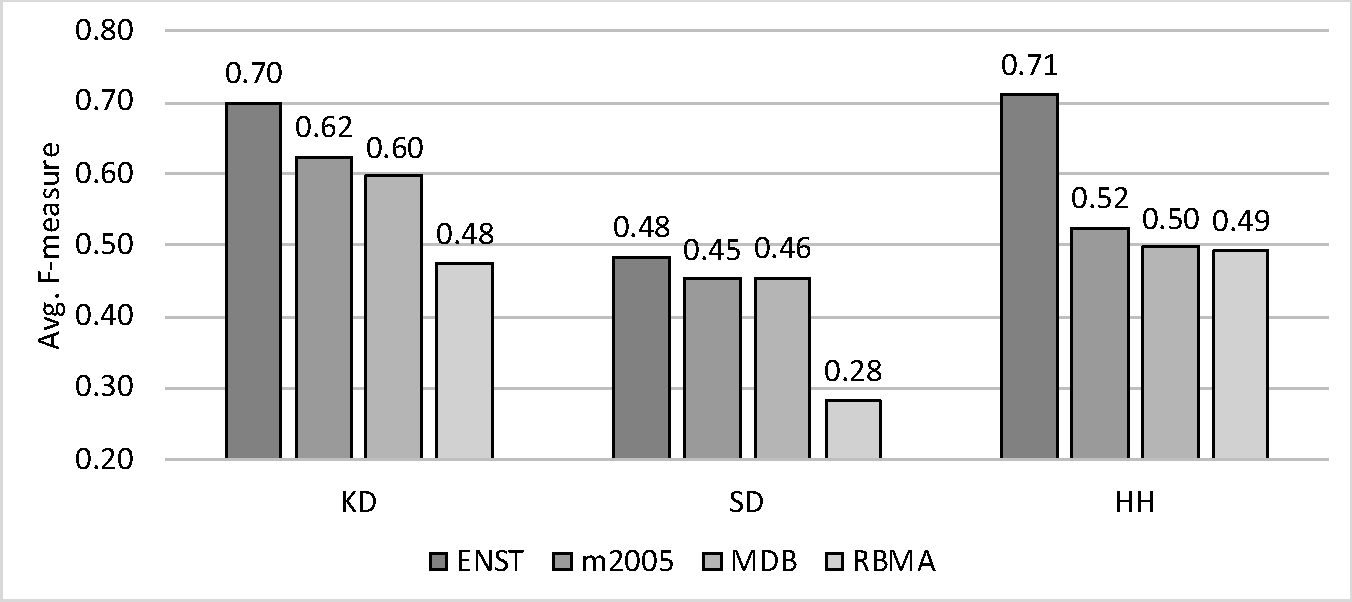
\includegraphics[width = \columnwidth]{./figs/avgAcrossDatasets.pdf}
\caption{The evaluation results of all labeled datasets with averaged F-measure across all systems.}
\label{fig:resultsAcrossDatasets}
\end{figure}

Based on these 9 systems, the following experiments are conducted:
\begin{compactenum}
\item [\textbf{E1:}]\textbf{Experiment 1} aims to examine the variance of the labeled datasets. For each dataset, the averaged F-measures across all 9 systems are reported. 
\item [\textbf{E2:}]\textbf{Experiment 2} aims to evaluate the usefulness of unlabeled data for \textit{Segment and Classify}-based ADT systems using the feature learning paradigm. For each system, the averaged F-measures across all the datasets are reported. 
\item [\textbf{E3:}]\textbf{Experiment 3} aims to evaluate the usefulness of unlabeled data for \textit{Separate and Detect}-based ADT systems using the student-teacher learning paradigm. For each system, the averaged F-measures across all the datasets are reported. \\
\end{compactenum}
Note that for feature learning paradigm, a cross-dataset validation process is performed (e.g., train on three datasets and test on the remaining one) in order to train the binary classifiers (see Sect.~\ref{subsec:featureLearning} for more details). For student-teacher learning paradigm, since the student model does not need additional labeled data for training, the cross-dataset validation is unnecessary. 

\subsection{Results}

% E1: averaged across systems: show the difficulty of the datasets
% need another table here
Figure~\ref{fig:resultsAcrossDatasets} shows the evaluation result of \textbf{E1}. On average, all systems tend to perform the best on \textit{ENST} and the worst on \textit{RBMA}. For some instruments, this gap can be as large as 22\% in F-measure. 
There are two possible reasons for the good performance on \textit{ENST}. First, as all systems have been developed and evaluated mostly on this dataset, there could be potential bias towards this dataset. Second, the \textit{ENST} dataset might be relatively simple compared with the others. A closer examination of the dataset shows the lack of singing voices and the dominance of MIDI synthesized accompaniments, which could potentially over-simplify the ADT problem. 
The relative poor performance on the \textit{RBMA} dataset might be related to its focus on EDM; the electronic drum sounds with strong audio effects could possibly increase the difficulty for ADT. This seems to be especially true in case of the SD.
Overall, the results show that the evaluated systems leave much room for optimization; since many of the parameters in these systems are not extensively tuned, this result is to be expected. However, this also reflects the challenge of building an ADT system that is easily generalizable. 
%Finally, the high variance across all the datasets suggests the possibility of being biased when relying on only one dataset; this also highlights the importance of evaluating ADT systems on multiple datasets.   

% E2: results of the feature learning systems
% trained is always better than random except hh
% sd always improved
\begin{table}[]
\centering
\resizebox{\columnwidth}{!}{%
%\footnotesize
%\begin{tabularx}{\columnwidth}{XXXXX}
\begin{tabularx}{\columnwidth}{ccccc}
\hline
\multicolumn{2}{l}{\textbf{Experiments}}             & \multicolumn{3}{l}{\textbf{Averaged F-measure}} \\ \hline
\textbf{Role} & \multicolumn{1}{l|}{\textbf{System}} & \textbf{HH}   & \textbf{BD}    & \textbf{SD}    \\ \hline
Baseline      & \multicolumn{1}{l|}{MFCC}            & 0.61          & \textbf{0.62}  & 0.40           \\
Baseline      & \multicolumn{1}{l|}{CONV-RANDOM}    & 0.61          & 0.54           & 0.39           \\
Evaluated      & \multicolumn{1}{l|}{CONV-AE}        & 0.61          & \textbf{0.62}  & \textbf{0.42}  \\
Evaluated      & \multicolumn{1}{l|}{CONV-DAE}       & 0.61          & 0.61           & \textbf{0.42}  \\ \hline
\end{tabularx}
}
\caption{Evaluation results of the feature-learning-paradigm-based systems.}%\comment{I don't like the ``proposed.'' Maybe just remove the Role? Also, adjust to column width}}
\label{tab:e2result}
\end{table}

\begin{table*}[t]
\centering
%\footnotesize
%\begin{tabularx}{\textwidth}{XcccXcXc}%{cccccccc}
\begin{tabularx}{\textwidth}{cccccccc}
\hline
\multicolumn{2}{c}{\textbf{Compared Systems}} & \multirow{2}{*}{\textbf{Inst.}} & \multirow{2}{*}{\textbf{Paradigm}} & \multicolumn{2}{c}{\textbf{Improvement}}    & \multicolumn{2}{c}{\textbf{Deterioration}}  \\ \cline{1-2} \cline{5-8} 
\textbf{Test}          & \textbf{Ref}         &                                      &                                    & \textbf{\# Files} & \textbf{F-measure Gain} & \textbf{\# Files} & \textbf{F-measure Loss} \\ \hline
CONV-AE               & MFCC                 & SD                                   & Feature Learning                   & 70/137            & 6.5\%                   & 40/137            & -4.6\%                  \\
FC-200                & PFNMF (SMT)          & HH                                   & S-T Learning                       & 78/137            & 13.8\%                  & 44/137            & -7.6\%                  \\ \hline
\end{tabularx}%
\caption{Significance check of the most improved pair from each paradigm.}
\label{tab:improvCheck}
\end{table*}

The results of \textbf{E2} are shown in Table~\ref{tab:e2result}. The following trends can be observed: first, the unlabeled data seems to be helpful in \textit{Segment and Classify}-based ADT systems. A direct comparison between CONV-AE and MFCC shows that the features learned from unlabeled data seem to slightly improve for SD while achieving equal performance on HH and BD. Second, the unsupervised training process is useful for deriving better features. Compared with CONV-RANDOM, both CONV-AE and CONV-DAE show improvements on nearly all instruments, indicating the advantage of the training process. Third, the DAE-inspired training process does not lead to improvements for ADT. This is shown by the almost equivalent results from CONV-AE and CONV-DAE. Since HPSS also introduces artifacts, it might not be the most ideal method for this task;  experimentation with other source separation algorithms might provide more insights. 
%\comment{yeah, but why not?}


% E3: results of the student-teacher systems
% discuss the varying dataset size vs. results
% criteria for selecting unlabeled data?
\begin{table}[]
\centering
%\footnotesize
\begin{tabularx}{\columnwidth}{XXXXX}
\hline
\multicolumn{2}{l}{\textbf{Experiments}}                    & \multicolumn{3}{l}{\textbf{Averaged F-measure}} \\ \hline
\textbf{Role} & \multicolumn{1}{l|}{\textbf{System}}        & \textbf{HH}    & \textbf{BD}    & \textbf{SD}   \\ \hline
Teacher       & \multicolumn{1}{l|}{PFNMF (SMT)}            & 0.47           & 0.61           & \textbf{0.45} \\
Teacher       & \multicolumn{1}{l|}{PFNMF (200D)}           & 0.47           & \textbf{0.67}  & 0.40          \\
Student       & \multicolumn{1}{l|}{FC-200}                & \textbf{0.56}  & 0.57           & 0.44          \\
Student       & \multicolumn{1}{l|}{FC-ALL}               & 0.53           & 0.59           & 0.42          \\
Student       & \multicolumn{1}{l|}{FC-ALL (ALT)} & 0.55           & 0.58           & 0.44          \\ \hline
\end{tabularx}
\caption{Evaluation results of the student-teacher-paradigm-based systems.}%\comment{Adjust to column width}}
\label{tab:e3result}
\end{table}


Table~\ref{tab:e3result} shows the results of \textbf{E3}. The general trends can be summarized as follows: first, the student-teacher learning seems to be useful for \textit{Separate and Detect}-based ADT systems as all students show a noticeable improvement on HH over the teacher models. This observation consolidates the preliminary finding reported in \cite{Wu2017}. Second, more unlabeled data do not necessarily lead to better results. For example, FC-200 and FC-ALL (ALT) both outperform FC-ALL on HH and SD. 
%While this result seems somewhat counter-intuitive, it may suggest that the noisy nature of the unlabeled data increases with the increasing amount of data. 
Since the student model is a simple feed-forward DNN, the lack of model capacity could limit its potential for further improvement as the data size grows. Experiments using other student models (e.g., CNNs and RNNs) would be necessary for confirmation.   
Third, the student models seem to struggle on BD. A detailed examination on the individual results from each dataset shows that teachers and students are mostly comparable on BD except for \textit{RBMA}. This is possibly due to the challenging nature of \textit{RBMA} as discussed in \textbf{E1}. However, further investigation might be needed before drawing conclusions. %\comment{do the results like much nicer when you remove rbma?}

% additional analysis goes here



% finally, compare two paradigms (pool the best systems from each)
% the differences between two systems are not statistically significant on all instruments
% definitely mention the additional need of labeled data in feature learning 
% so student  teacher is slightly favored for it requires less labeled data

The results of \textbf{E2} and \textbf{E3} show that feature learning and student-teacher learning paradigms are able to improve the performance on SD and HH, respectively. In light of these results, an interesting question is: ``Are these improvements significant?'' In an attempt to answer this question, two pairs of systems are selected for further analysis. Each pair consists of the best baseline and the best evaluated system of each paradigm. A t-test is performed on each pair by comparing their results on all 137 files. Both pairs have shown significant improvements with $p \ll 0.05$ for both t-tests. Furthermore, the number of improved and deteriorated files is calculated. The results, shown in Table~\ref{tab:improvCheck}, show a positive trend: the number of improved files is, in both cases, greater than the number of deteriorated files. Moreover, the averaged F-measure gains are also higher than the averaged F-measure loss for both pairs.  

Comparing the pairs on Table~\ref{tab:improvCheck} with each other, the improvements on HH from the student-teacher learning paradigm seems to be more substantial. To further investigate the cause of this improvement, one example from the \textit{ENST} dataset, which has the largest F-measure gain among all files, is selected. The HH activation functions generated from both teacher and student model are shown in Fig.~\ref{fig:exampleActiv}. Compared to the teacher's activation function, the student's activation function is sharper and cleaner, demonstrating the benefit of this paradigm.

% example from ENST
\begin{figure}
\centering
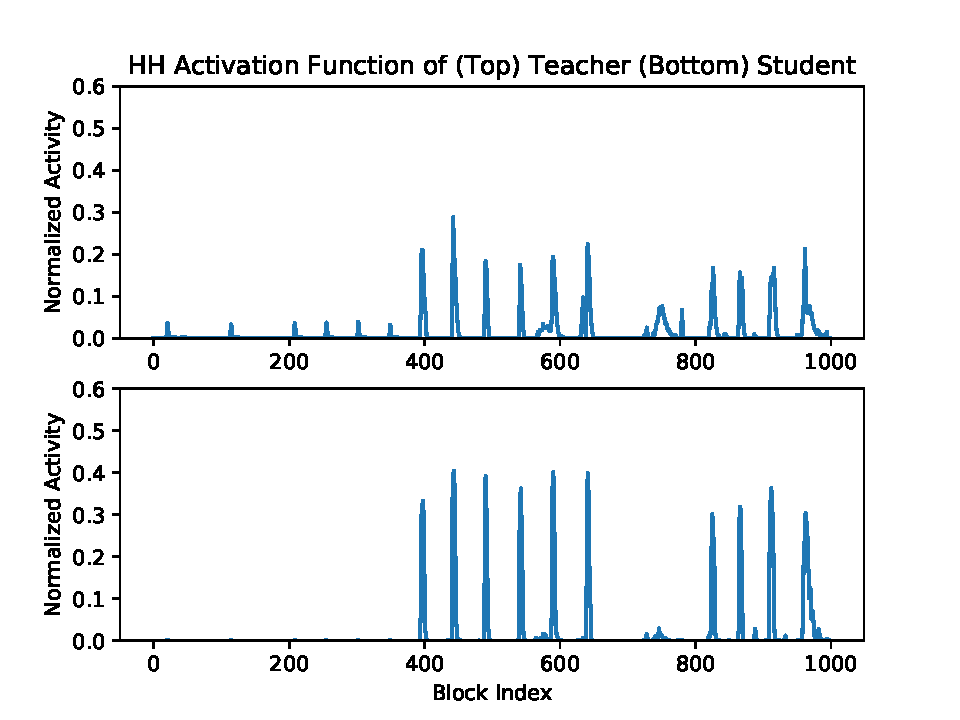
\includegraphics[width = \columnwidth]{./figs/example_activ.pdf}
\caption{Example of the (top) teacher's and (bottom) student's HH activation function in comparison.}
\label{fig:exampleActiv}
\end{figure}


\section{Conclusion}
\label{sec:conc}

In this paper, we discussed the data challenge in ADT and investigated two approaches to address this challenge by considering both labeled and unlabeled data. First, we compared system performance on the multiple existing labeled datasets in an unified setting. The results indicate a potential bias of relying on one dataset and highlight the necessity of including more datasets in the future ADT evaluation. Furthermore, we evaluated the usefulness of unlabeled data for two major types of ADT systems via two different learning paradigms, feature learning and the student-teacher learning approach. For both paradigms, we got encouraging (and statistically significant) results demonstrating the potential of achieving better performance than the baseline systems on different drum instruments.

These results, while suggesting the need for additional labeled data in the field of ADT, also encourage the exploration of incorporating unlabeled data in the training. 
Possible future directions include
\begin{inparaenum}[(i)]
	\item the evaluation of various methods for unsupervised feature learning such as Sparse Coding \cite{Raina2007a} and Deep Belief Networks \cite{Hamel2010},
    \item the evaluation of different combinations of teacher and student models, for example, the combination of different types of DNN either as teachers or students; the identification of suitable architectures for these roles could also be an interesting direction, and
    \item the application of outlier detection \cite{Lu2016} approaches to filter out noisy unlabeled data.   
\end{inparaenum} 

% For bibtex users:
\bibliography{cw_ismir2018_ref}

% For non bibtex users:
%\begin{thebibliography}{citations}
%
%\bibitem {Author:00}
%E. Author.
%``The Title of the Conference Paper,''
%{\it Proceedings of the International Symposium
%on Music Information Retrieval}, pp.~000--111, 2000.
%
%\bibitem{Someone:10}
%A. Someone, B. Someone, and C. Someone.
%``The Title of the Journal Paper,''
%{\it Journal of New Music Research},
%Vol.~A, No.~B, pp.~111--222, 2010.
%
%\bibitem{Someone:04} X. Someone and Y. Someone. {\it Title of the Book},
%    Editorial Acme, Porto, 2012.
%
%\end{thebibliography}

\end{document}
